\chapter{Results}\label{Results}


\section{Gamma-/Hadron-Separation}\label{Gamma-/Hadron-Separation}

With the previously mentioned datasets and parameters, the distribution of the predicted gammaness
on the cross-validated dataset is illustrated in figure \ref{fig:gh_sep}.

\begin{figure}
    \centering
    \captionsetup{width=0.9\linewidth}
    \includegraphics[page=2, width=.9\textwidth]{../analysis/plots/cross_val_sep_perf_plot.pdf}
    \caption{Distribution of the predicted gammaness on the cross-validated training sets.
	    The two populations (Proton and Gamma, marked in blue and orange), can be separated 
	    to a certain degree.
        A perfect prediction would show no overlap between the distributions.}
    \label{fig:gh_sep}
\end{figure}

To evaluate the resulting performance of the model, the ROC-curve, precision, recall and
$F_{\num{0.10}}$-score get calculated. 
The ROC-curve is shown in figure \ref{fig:gh_roc}, with the model achieving an AUC of 
$\approx \num{0.89}$.

\begin{figure}
    \centering
    \captionsetup{width=0.9\linewidth}
    \hspace*{0.15\textwidth}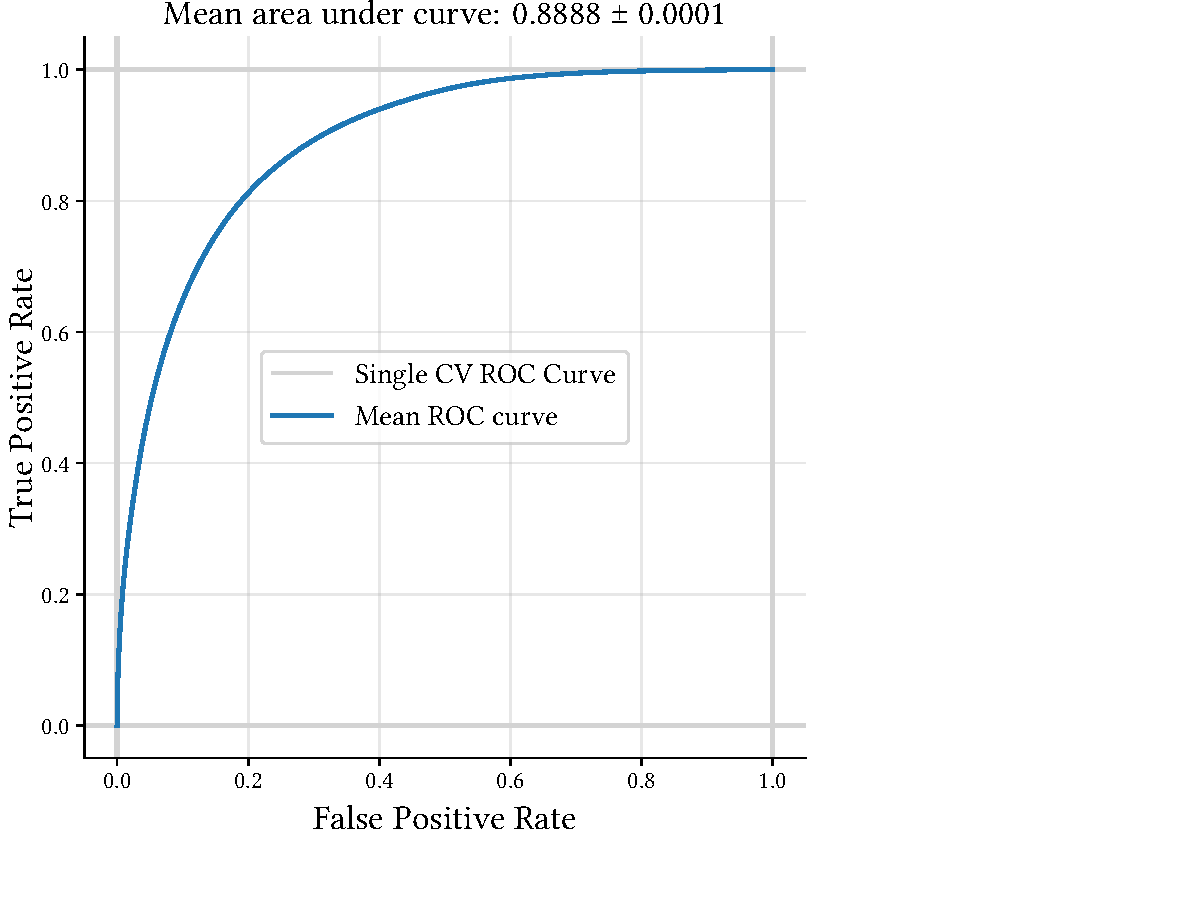
\includegraphics[page=1, width=.9\textwidth]{../analysis/plots/cross_val_sep_perf_plot.pdf}
    \caption{ROC-curve for the gamma/hadron separation on the cross-validated training sets.
    A mean AUC of \num{0.8858 \pm 0.0002} gets obtained with the trained model.
    The five ROC-curves from the individual cross validation steps show almost no deviation.}
    \label{fig:gh_roc}
\end{figure}

Figure \ref{fig:gh_fscore} shows the precision, recall and $F_{\num{0.10}}$-score over
the prediction threshold.
For the hadroness cut we choose the maximum of the $F_{\num{0.10}}$-score
at $\approx \num{0.82}$

\begin{figure}
    \centering
    \captionsetup{width=0.9\linewidth}
    \includegraphics[page=3, width=.9\textwidth]{../analysis/plots/cross_val_sep_perf_plot.pdf}
    \caption{Precision, recall and $F_{\num{0.10}}$-score for the gamma/hadron separation model on the 
    cross-validated training sets.
    In accordance to the distribution in figure \ref{fig:gh_sep}, the precision improves up
    to $\approx \num{0.97}$, which marks the hight predictions for gamma events.
    The recall on the other hand gets worse with higher threshold as legitimate gamma events,
    that achieved a low prediction get removed. 
    The maximum $F_{\num{0.10}}$-score is achieved at a prediction threshold
    of $\approx \num{0.82}$, which is where the hadroness cut will be applied.}
    \label{fig:gh_fscore}
\end{figure}


The feature importance, as calculated via sklearn, is shown in figure \ref{fig:gh_features}.
\begin{figure}
    \centering
    \captionsetup{width=0.9\linewidth}
    \hspace*{-0.15\textwidth}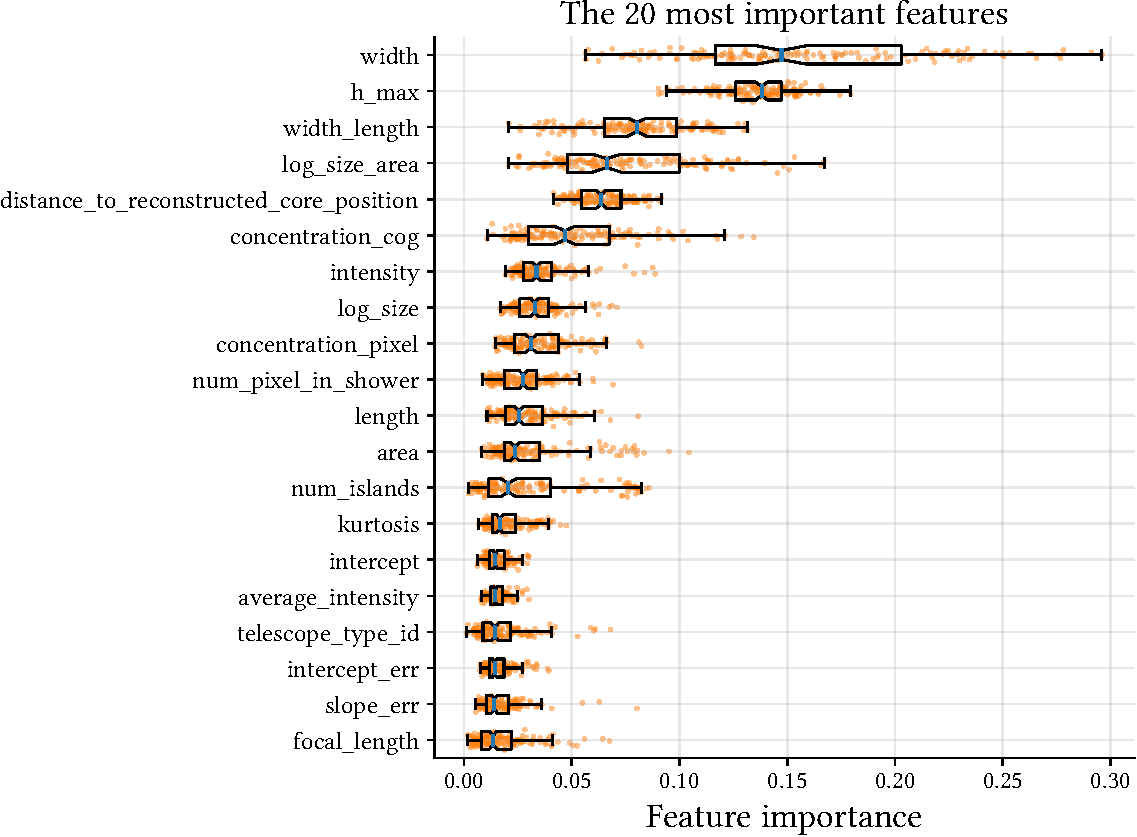
\includegraphics[page=1, width=.9\textwidth]{../analysis/plots/separation_features.pdf}
    \caption{Feature importance for the gamma/hadron separation model evaluated on the cross-validated dataset.
    The separation seems to be based mostly on the description of the main shower ellipse, especially its width and length.
    From the stereoscopic features the predicted interaction height heavily influences the predictions.
    The number of islands only rarely provides a lot of information, which might indicate that our chosen cleaning 
    removes most additional clusters. -> VERTEILUNG DER ISLANDS ALS KONTROLLE PLOTTEN?}
    \label{fig:gh_features}
\end{figure}
